    { \footnotesize
    \begin{figure}
    \centering
    %
    \begin{subfigure}{.27\textwidth}
        $
        \begin{array}{l}
          \kw{twoPathsWhile}(n, m) \triangleq \\
        \clabel{ \assign{i}{n} }^{0} ;
        \clabel{ \assign{j}{0} }^{1} ; \\
        L_2:    \ewhile ~ \clabel{i > 0}^{2} ~ \edo ~ \\
            \qquad \Big(
              \eif(\clabel{j < m}^{3}, \\
              \qquad \ethen  \clabel{\assign{j}{j + 1}}^{4}; \\
              \qquad \qquad \clabel{\assign{i}{i - 1}}^{5},\\
              \qquad \eelse \clabel{\assign{j}{0}}^{6});
              \Big)
            \end{array}
            $
\vspace{-0.2cm}
\caption{}
\end{subfigure}
\begin{subfigure}{.71\textwidth}
\begin{subfigure}{.67\textwidth}
\begin{centering}
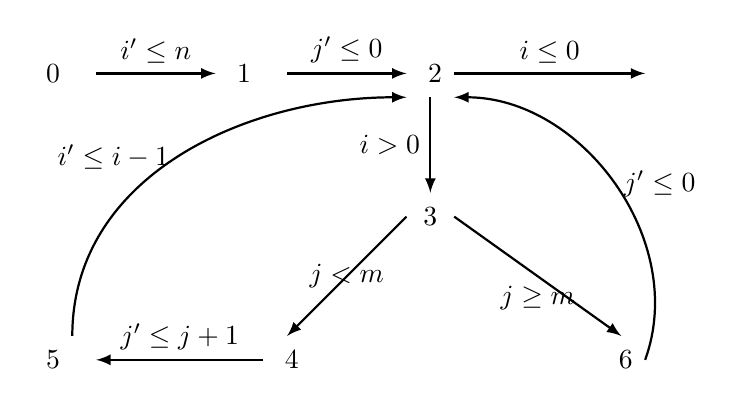
\begin{tikzpicture}[scale=\textwidth/20cm,samples=200]
    \draw[] (-8, 10) circle (0pt) node{{ $0$}};
    \draw[] (-4, 10) circle (0pt) node{{ $1$}};
    \draw[] (0, 10) circle (0pt) node{{ $2$}};
    \draw[] (0, 7) circle (0pt) node{{$3$}};
    \draw[] (-3, 4) circle (0pt) node{{ $4$}};
    \draw[] (-8, 4) circle (0pt) node{{ $5$}};
    \draw[] (4, 4) circle (0pt) node{{ $6$}};
    % Counter Variables
    \draw[] (5, 10) circle (0pt) node {\textbf{$\lex$}};
    %
    % Control Flow Edges:
    \draw[ thick, -latex] (-7, 10)  -- node [above] {$i' \leq n$}(-4.5, 10);
    \draw[ thick, -latex] (-3, 10)  -- node [above] {$j' \leq 0$}(-0.5, 10);
    \draw[ thick, -latex] (0, 9.5)  -- node [left] {$i > 0$} (0, 7.5) ;
    \draw[ thick, -latex] (0.5, 7)  -- node [below] {$ j \geq m $}  (4, 4.5);
    \draw[ thick, -latex] (-7.5, 4.5)  to  [out=90,in=180]  node [left] {$i' \leq i - 1$ }(-0.5, 9.5);
    \draw[ thick, -latex] (4.5, 4)  to  [out=70,in=0]   node [right] {$j' \leq 0 $}(0.5, 9.5);
    \draw[ thick, -latex]  (-0.5, 7) -- node  {$j < m$}  (-3, 4.5) ;
    \draw[ thick, -latex]  (-3.5, 4) -- node [above] {$j' \leq j + 1$}  (-7, 4) ;
    \draw[ thick, -latex] (0.5, 10)  -- node [above] {$i \leq 0$}  (4.5, 10);
  \end{tikzpicture}
        \caption{}
\end{centering}
\end{subfigure}
{\small
\begin{subfigure}{.3\textwidth}
\begin{centering}
        $\tpath_0 = 0 \to 1 \to 2$ \\
        $\tpath_2 = 2 \to 3 \to 6 \to 2$ \\ 
        $\tpath_1 = 2 \to 3 \to 4 \to 5 \to 2$ \\
        $\tpath_3 = 2 \to \lex$
        \caption{}
\end{centering}
\end{subfigure}
}
{\small
\begin{subfigure}{.8\textwidth}
\begin{centering}
    $
    \tpath_0 ; 
    \rpchoose{2: \rprepeat_2(\rprepeat_1(\tpath_1); \tpath_2), 
    2: \rprepeat_1(\tpath_1)}; \tpath_3.
    $
\end{centering}
\end{subfigure}
}
\end{subfigure}
\vspace{-0.2cm}
\caption{
    (a) The two paths loop example,
    (b) the Abstract Transition Graph for $\kw{twoPathsWhile}(n, m)$,
    (c) the Simple Transition Paths of $\kw{twoPathsWhile}(n, m)$.}
    \vspace{-0.5cm}
        \label{fig:whileTwoCounters-overview}
    \end{figure}
    }


